\documentclass{article}
\usepackage[utf8]{inputenc}
\usepackage{graphicx}
\usepackage{amsmath}
\usepackage{booktabs}
\usepackage{textcomp}
\usepackage{multirow}
\usepackage{color}


\begin{document}
\title{Aufgabenblatt 1}
\author{Christian Müller, Ralph Krimmel \& Sebastian Albert }

\maketitle


\section*{Assignment 1 - Data Center Infrastructure}

\subsection*{a}
	The core elements of a data center are described in the following part and can be seen in figure \ref{fig:coredata} :

	\begin{figure*}[t]
		\begin{center}
			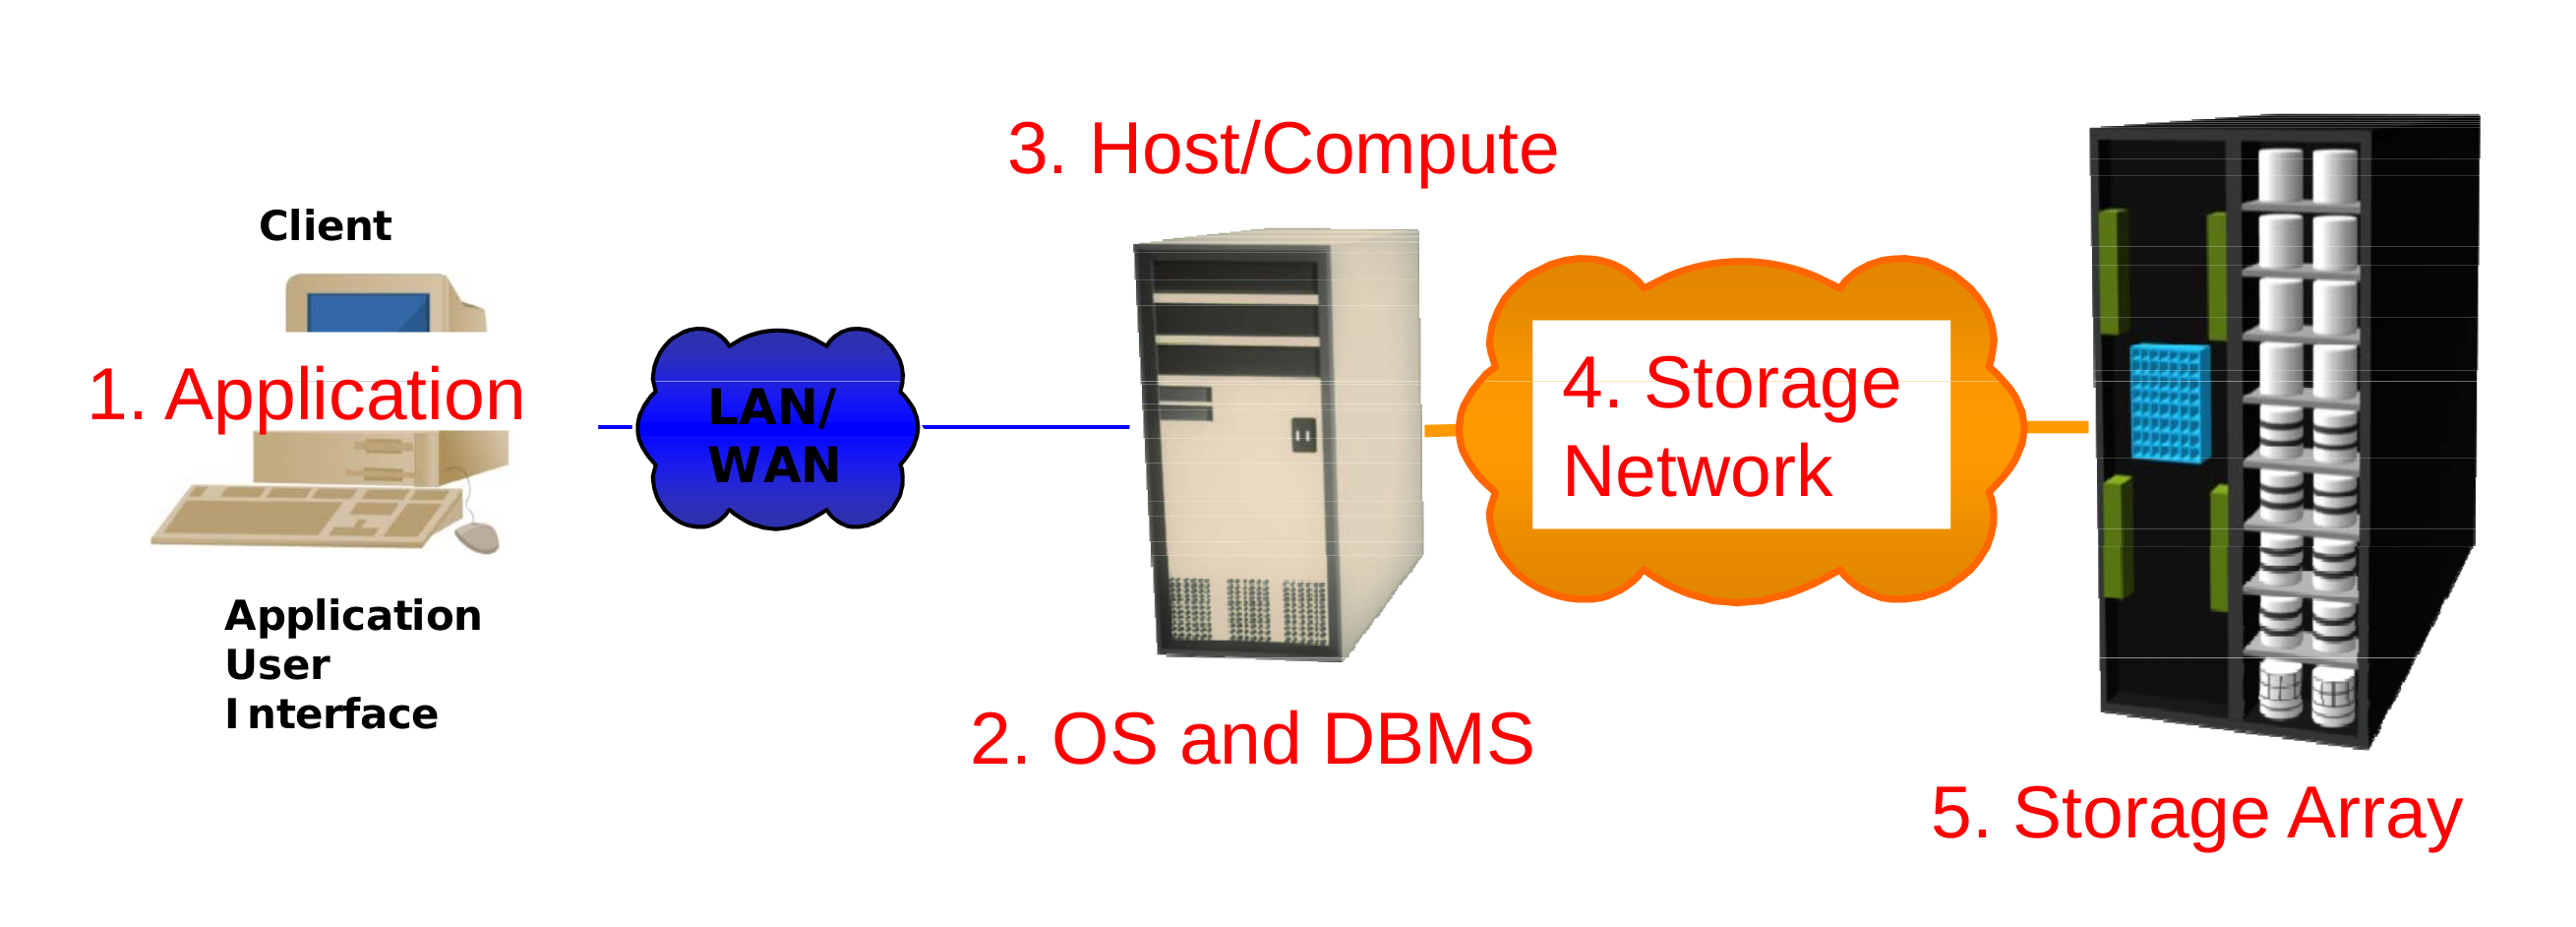
\includegraphics[width=\textwidth]{pic/datacenter.png}
		\end{center}
		\caption{The core elements of a data center.}
		\label{fig:coredata}
	\end{figure*}

	\begin{description}
		\item[Application] \hfill \\
			Software that provides the logic for computing operations.
			It is characterized by its I/O profile,
			which describes how the application reads and writes data.
			Typical categories are read or write intensive applications
			or ones that have more sequential or random read and write operations.
			Another factor is the typical I/O size.
			Applications can be isolated by virtualization,
			which avoids conflicts and can enhance data protection.\\
			In the hospital example the application is the access to the X-Ray data.

		\item[Database management system (DBMS)] \hfill \\
			Databases store structured data in tables that have can have relations with each other.
			DBMS controls the creation, maintance and use of the databases.
			These systems can be querried by applications for certain information.\\
			The Orcale database is the DBMS in the given example.
			
		\item[Host or Compute] \hfill \\
			A ressource that runs an application with the its computing components.
			It consist of a physical machine and the operating system.
			They enable the application to run by supplying CPU, memory and I/O devices on the hardware side
			and operating system, device driver, file system and volume manager on the software side.
			Hosts can be virtualized to enhance the usability of the physical entity.
			Examples for hosts are servers, clusters, laptops and desktops.\\
			In the hospital example, the host is the UNIX server.

		\item[Network] \hfill \\
			The network interconects the hosts and the storage.\\
			In the given hospital example it is established by the Gigabit Ethernet backbone.

		\item[Storage] \hfill \\
			The storage provides access to the data stored in the data center.
			The storage array with 6 TB of usable capacity represents the storage in the given hsopital example.

	\end{description}

	In a hospital the requirements are very high,
	as the life of humans can be endangered if the infrastructure is not working.
	Very important is the \emph{availability} and \emph{performance} of the data storage,
	to ensure every patient gets the correct treatment the moment he needs it.
	One also has to make sure that the data is not altered and can not be accessed by unauthorized persons,
	so \emph{integrity} and \emph{confidentiality}, \emph{data protection} and \emph{security} are also important concepts.
	As the amount of data will increase daily in hospital,
	the data center must be able to store these increasing amounts of data and scale along.

\subsection*{b}

\end{document}
